% Figura 3 - choropleth do deserto de distancia. src: 12_fig_desert_maps.py
\begin{figure}[t]
\centering
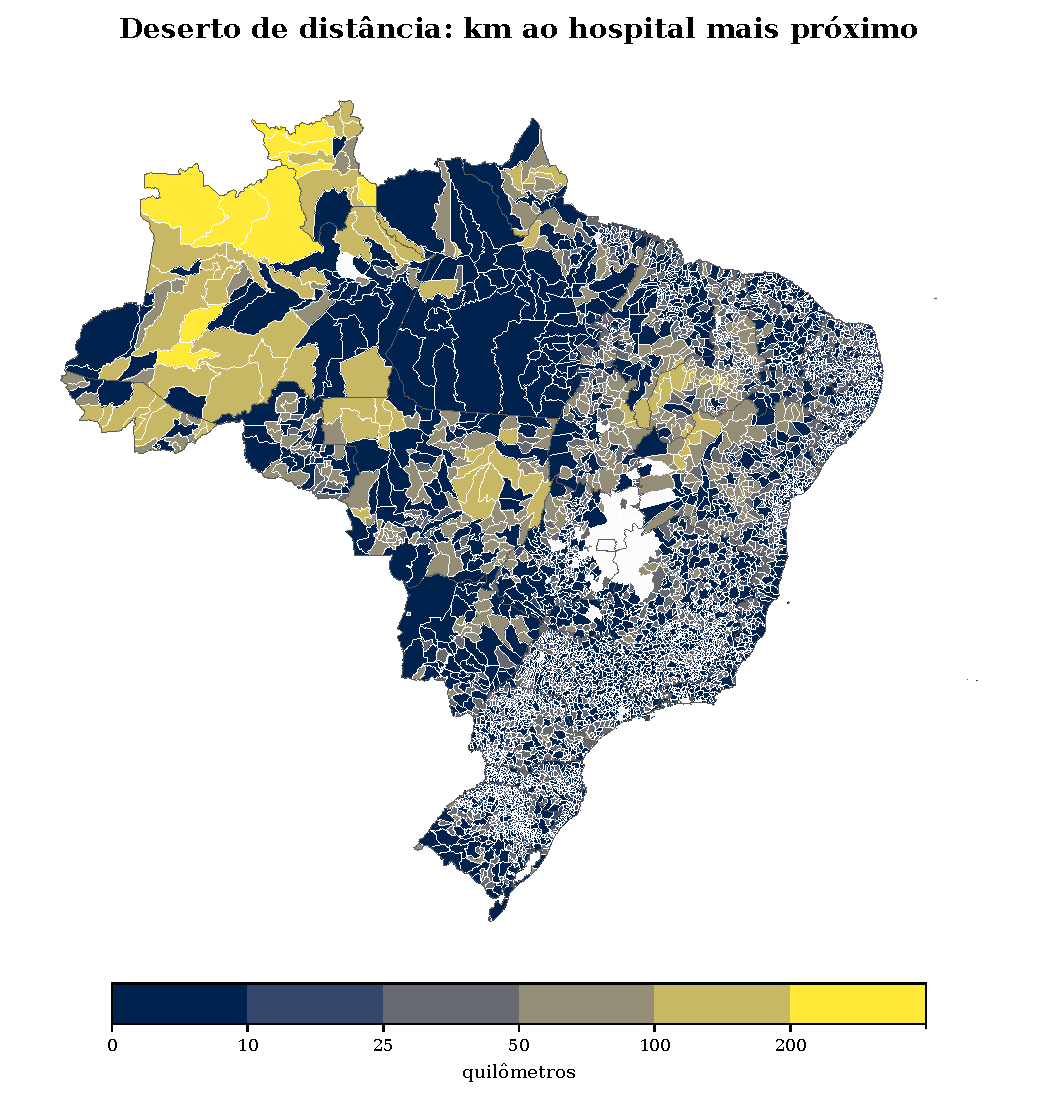
\includegraphics[width=0.86\linewidth]{../04_figures/fig3_distance_map.pdf}
\caption{\textbf{Deserto de distância: quilômetros ao hospital ativo mais
próximo.} Cada município colorido pela distância de centroide ao hospital com
leito mais próximo, 2015--2022. A escala de cores (em km) é idêntica à da
Figura~\ref{fig:flow_map}, permitindo comparação direta. A maior parte do país
aparece em tons escuros (perto); o isolamento de distância concentra-se na
Amazônia, onde, contudo, a malha rodoviária não representa o deslocamento real
por rio. Projeção Brasil Polyconic (EPSG:5880). Fonte: CNES, OSRM, IBGE.}
\label{fig:distance_map}
\end{figure}
